\chapter{Common Parallel Patterns}

A pattern is a tested solution to a certain kind of problem under some conditions. Here we have summarised several common patterns in parallel computing and listed them below.

\section{Embarrassingly Parallel}

Embarrassingly parallel looks more like a problem rather than a pattern. It deals with problems where separating the original problem into smaller ones takes very little or no effort at all. This happens when no communication or dependence exists among separated small problems, for example, if all sub-problems just need to do the same operation and they are independent from each other.

Some problems can be turned into embarrassingly parallel easily. For example, if all sub-problems dependent only on global data structure, then just replicate global data to all sub-problems thus being embarrassingly parallel.

\section{Pipeline}

Pipeline is a classic pattern or architecture. We have already introduced hardware pipelines inside processor cores in section 3.1.2, and here we will introduce software pipeline pattern or architecture, for parallel purpose.

Software pipeline is composed of several threads or processes, which depends on implementation. A continuous data stream flows into the first thread or process as input and pass corresponding output as input to next thread or process. It continues so that every thread or process can do certain action on part of data simultaneously.

The most popular software pipeline should be Unix pipeline. It composes Unix commands into a pipeline with simple $\mid$ signs, which makes Unix shell extremely strong and flexible. It is implemented with multiple processes.

\section{Master-Slave}

Master-Slave pattern or architecture may be the easiest one to implement on distributed environment. In a Master-Slave structure, a master process takes care of the essential serial part of the whole parallel program, while several slaves execute the paralleled workload. Any slave who finishes current workload will inform the master and wait for master's response, like starting a new task. The figure later in this section is a brief illustration of how master-slave pattern works.

\begin{figure}[ht]
\centering
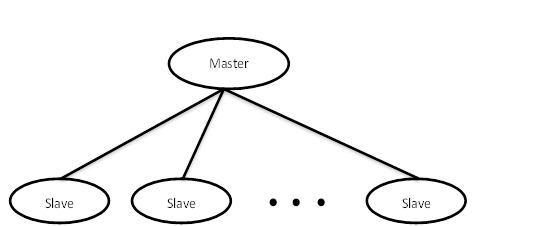
\includegraphics[width=120mm]{master-slave-brief.png}
\caption{A brief illustration of master-slave pattern}
\end{figure}

Since master does serial part and takes extra cost like coordination, it is very easy to become the bottle neck of whole parallel program, although get multi-levelled. We will give a deeper analysis in the next chapter since we adopted this pattern or architecture in our implementation.

Master-Slave pattern is a high-level abstract pattern. There're many specific instances, like fork-join. 

Fork-join maybe the simplest instance of master-slave structure. In this instance the master will start or fork many slaves first, then wait for or join the finish point of all the slaves, with a barrier generally.

Master-Slave structure is so high-level abstract that even the Hadoop map-reduce, which we will introduce in the next section, has a master-slave structured underlay.

\section{Map-Reduce}

This pattern has become hot in recent years due to Google's publication \cite{google-map-reduce} followed by Apache's open source implementation named Hadoop. The key idea is to first split original data set into small pieces and perform the same operation called "map" on these data pieces, turning every data piece into key-value pair format. Then perform the same operation called "reduce" on the intermediate key-value pairs and finally combined them together to get final result.

It is much more than a theoretical pattern because of the Hadoop framework. It has covered many parallel implementation details so that programmer can focus on the business logic part, say, "map" operation and "reduce" operation. The only left difficult point for programmers is how to fit original problem into such two steps.

\section{Parallel Pattern Conclusion}

Parallel patterns listed above are common and intuitive. They take advantage of data decomposition and functional decomposition, but rely heavily on the natural presentation of original problem and fit problem into suitable patterns.

To expose better parallelism, advanced tricks are involved like Fast Fourier Transform to take advantage of specific domains, which are not that common any more.

Besides, patterns are more art than science. It is not necessary to stick strictly to some pattern as long as the problem get solved.
